\documentclass[conference]{IEEEtran}
\usepackage[T1]{fontenc}
\usepackage[utf8]{inputenc}
\usepackage{amsmath,amssymb,graphicx,booktabs,url}
\usepackage[hidelinks]{hyperref}
\urlstyle{same}
\def\UrlBreaks{\do\/\do\-\do\_\do\.}
\begin{document}
\title{Stress-Testing Mask Augmentation: Threshold Effects and Unseen-Channel Failures in Imbalanced Maintenance Data}
\author{\IEEEauthorblockN{Machine Learning Course Project}}
\maketitle
\begin{abstract}
A fault classifier may face missing measurements after deployment even when its clean-test accuracy is high. We study whether inexpensive group-outage augmentation improves minority-fault detection and transfers to outages excluded from development. The experiment uses real Scania APS records and synthetic AI4I data, three fixed split seeds, four training configurations, and separate clean-only and outage-aware threshold selection. Across clean data and three anticipated outages, group-augmented boosting increases mean positive-class F1 from 0.8359 to 0.8435 on APS and from 0.5610 to 0.6006 on AI4I. The APS improvement has a conditional bootstrap interval spanning zero. Transfer is weaker: under an untrained rotational-speed outage, AI4I F1 falls to 0.223, below standard boosting's 0.441. A random-cell masking control transfers better to the two untrained AI4I outages; an exploratory clean-repeat control also outperforms targeted masking on the AI4I primary endpoint. These results support testing both outage coverage and threshold policy before adopting masking augmentation. We release fitted models, predictions, split indices, and analysis code; the contribution is controlled empirical evidence, not a new learning algorithm.
\end{abstract}
\begin{IEEEkeywords}
missing-data shift, fault classification, class imbalance, gradient boosting, decision thresholds
\end{IEEEkeywords}

\section{Introduction}
Industrial classifiers often predict from several measurements collected together. A missing measurement can change the classifier's input distribution without changing the equipment's condition. A model evaluated only on ordinary held-out rows may therefore give an incomplete picture of deployment performance. Missingness shift is already a research problem with both theoretical treatments and empirical benchmarks \cite{zhou23b,cheng25e}. The practical question is which inexpensive mitigation is justified for a particular monitoring task.

This paper examines group-outage augmentation: fit a classifier on the original training rows and copies with selected measurement groups removed. We ask whether gains on anticipated outages survive separating the training procedure from its decision threshold, and whether those gains extend to different full-group outages. We use APS Failure at Scania Trucks as the primary dataset and AI4I as a secondary synthetic case. Both tasks classify recorded conditions. Neither experiment estimates remaining useful life or establishes warning time before a future failure.

Our contributions are:
\begin{itemize}
\item A reproducible, two-dataset protocol that reserves two full-group outages from deliberate augmentation and threshold selection, with all channel ranking computed on training rows.
\item A training-by-threshold comparison, including a random-cell control with a matched selected-cell budget. This distinguishes changes in representation from changes in the operating point.
\item Evidence of a transfer boundary: modest anticipated-outage gains do not imply protection against untrained outages. The released artifacts retain negative results, conditional uncertainty, and an exploratory redundancy audit.
\end{itemize}
These are empirical contributions. We do not claim that masking, boosting, threshold optimization, or feature-loss stress tests are new. The study's scope is the controlled combination evaluated here; it does not establish global methodological novelty or state-of-the-art performance.

\section{Literature Review}
\subsection{Reconstructing missing inputs}
Muzellec \emph{et al.} optimize an optimal-transport discrepancy between batches for imputation \cite{muzellec20a}. Their experiments use 23 UCI datasets and evaluate MAE, RMSE, and Wasserstein distance (PDF pp. 6--9). These endpoints measure reconstruction quality; they do not directly answer whether a fault detector retains minority-class F1 after a new whole-channel outage.

HyperImpute searches over conditional models inside an iterative imputation loop \cite{jarrett22a}. Its main experiments use 12 UCI datasets with simulated missingness and report RMSE and Wasserstein distance (PDF pp. 3--6). Its column-wise model search is useful when reconstruction matters, but introduces a different computational objective from fitting a single small classifier. We therefore do not treat an imputation score as a substitute for classification performance.

EGG-GAE learns graph connectivity for tabular imputation and evaluates downstream random-forest accuracy as well as reconstruction \cite{telyatnikov23a}. Its surrogate corruption is MCAR, and its experiments cover MCAR, MAR, and MNAR mechanisms (PDF pp. 6--7). Appendix B reports, for example, 81.71\% $\pm$ 0.56 accuracy on Adult for EGG-GAE at 20\% MCAR (PDF p. 15). That result belongs to its own dataset, downstream model, and protocol. It is not a baseline score for APS or AI4I.

\subsection{Prediction and the assumptions behind missingness handling}
Zhou \emph{et al.} study domain adaptation under missingness shift, including a source-data masking adjustment \cite{zhou23b}. Their discussion explicitly reports that adjustment can fail when assumptions do not hold: on their real eICU comparison, the unadjusted source predictor gives the highest AUROC and average precision (PDF pp. 8--9). This is a direct reason to retain an unmodified baseline. Their redundant-feature example also shows that an expressive source model can perform well without adjustment.

Ayme \emph{et al.} analyze naive imputation through random-feature models and derive conditions under which its approximation bias is small \cite{ayme24a}. Their central setup uses squared prediction risk, with assumptions on feature generation and missingness (PDF pp. 3--8). These results caution against assuming that a more elaborate imputer must improve prediction. They do not give guarantees for our boosted, imbalanced classifiers.

Reyero Lobo \emph{et al.} analyze perceptron, logistic, and LDA classifiers under missingness \cite{lobo25a}. Their experiments show that apparently simple methods can behave differently from what broad model labels suggest, and that pattern-specific classifiers have limited data in small samples (PDF pp. 7--8). We include an indicator-augmented logistic model as a transparent reference, while recognizing that its linear decision function can be inadequate for nonlinear fault mechanisms.

\subsection{Avoidance, feature loss, and evaluation protocol}
MINTY reduces dependence on unavailable variables through disjunctive rules and a missingness-reliance penalty \cite{stempfle24a}. Its evaluated tasks are regression, and its synthetic MCAR setup uses the same mechanism in training and testing (PDF pp. 6--9). The later missingness-avoiding framework extends this principle to trees, tree ensembles, and sparse linear models \cite{stempfle25a}. It assumes a fixed joint distribution in its problem statement and explicitly identifies distribution shift as a limitation (PDF pp. 3, 6, 9). These works establish that reducing reliance and surviving a changed availability pattern are different questions.

TabFSBench already studies feature deletion, importance-ranked shifts, and multiple tabular model families \cite{cheng25e}. Its classification evaluation emphasizes accuracy and ROC-AUC (PDF pp. 3--6). Consequently, simply deleting features or comparing trees with linear models would not establish novelty. Our narrower experiment centers on positive-class F1, two deliberately untrained outage groups, a matched-cell training control, and a separate decision-threshold factor.

Cai and Ye show that training/validation protocols can materially affect performance under temporal shift \cite{cai25j}. Their study concerns time, not our availability interventions (PDF pp. 4--7). It reinforces the need to specify exactly which information is available for model selection. We make no temporal-generalization claim from random AI4I splits.

\subsection{Research gap and questions}
The gap addressed here is practical evidence for selecting a low-cost outage mitigation under class imbalance, rather than the discovery of feature shift itself. We ask:
\begin{enumerate}
\item Does targeted group masking improve F1 over clean data and anticipated outages relative to unaugmented boosting?
\item How much of any improvement depends on threshold selection, and does matched random-cell masking perform similarly?
\item Does the improvement transfer to full-group outages excluded from deliberate masking and threshold selection?
\end{enumerate}
The third question is essential: a method that performs well only on the outage identities encoded during development should not be advertised as general protection against missing sensors. The ten-paper review is targeted, covers 2020--2025, and is not an exhaustive survey through 2026. Page-grounded notes and publisher-mirror identifiers accompany the artifact.

\section{Experimental Setup}
\subsection{Datasets and provenance}
APS \cite{apsdata} contains 60,000 source rows, including 1,000 positives, and an official 16,000-row test set, including 375 positives. Here, ``clean'' means no additional masking; APS retains its natural missing values. There are 170 numerical features with anonymized names and natural missingness: 8.33\% of source cells and 8.41\% of test cells. The positive class concerns the APS component; the negative class concerns other component failures, so ``negative'' does not mean a healthy truck. The original dataset description defines a diagnostic cost of $10FP+500FN$.

AI4I \cite{ai4idata} contains 10,000 synthetic records with 339 machine-failure labels. We use five numerical measurements and one-hot encode product type into three columns. Identifiers and the five failure-mode indicator columns are excluded. Those indicators describe the target's failure types and would provide inappropriate information for our intended task. The resulting input has eight columns and no original missing cells.

Files were acquired from public GitHub mirrors pinned to commits, with SHA-256 checksums. The APS source description and original UCI source links are retained. We do not redistribute raw tables or infer their licensing from a mirror's code license. An exact-row audit finds no duplicate feature rows within either source and no overlap between APS source and official test features.

\subsection{Splits and training budget}
For each seed in $\{11,29,47\}$, APS source rows are stratified into 48,000 training and 12,000 validation rows; its official test set remains fixed. AI4I uses stratified 60/20/20 partitions: 6,000 training, 2,000 validation, and 2,000 test rows. Its test partitions differ across seeds. Imputation, scaling, and group ranking use training rows only. Augmented copies remain in the training partition.

The experiment runs on CPU with at most four numerical-library threads, Python 3.12.14, scikit-learn 1.8.0, NumPy 2.3.5, and pandas 2.2.3. Settings were fixed in a protocol file before fitting, and its hash appears in each run manifest. This is an internally frozen protocol, not an externally registered study. We perform no test-driven hyperparameter search.

\subsection{Models and controls}
The three principal models are balanced logistic regression, standard histogram gradient boosting (HGB), and group-augmented HGB (Group-HGB). Logistic inputs receive signed $\log(1+|x|)$ transformation, training-median imputation, standardization, and missingness indicators for all columns. Its L2 penalty uses $C=1$ with at most 1,500 iterations.

Every HGB fit uses 160 rounds, learning rate 0.08, at most 15 leaves, minimum leaf size 30, L2 regularization 1, native NaN handling, and balanced class weights. Early stopping is disabled, avoiding an internal split of correlated augmented copies. Cell-HGB provides an additional random-cell augmentation control. A majority classifier is retained in the machine-readable results. These are controlled scikit-learn baselines, not reproductions of published paper-specific implementations.

\section{Proposed Methodology}
\subsection{Training-only group ranking}
Let $G$ denote a set of input columns. APS columns with the same prefix before the underscore form one group, giving 107 groups; these are measurement-variable proxies, not verified physical sensors. Each AI4I numerical measurement forms a group; product-type columns are not artificially removed.

For numerical feature $j$, compute
\begin{equation}
 d_j=\frac{|\mu_{j,1}-\mu_{j,0}|}{\max(s_j,10^{-8})},\qquad d_G=\max_{j\in G} d_j,
\end{equation}
where class means and the overall standard deviation are calculated over observed training entries. Undefined scores become zero. Sort groups by descending $d_G$, breaking ties by name. The top three define development outages; ranks four and five define untrained full-group outages. Ranking is a simple availability-stress heuristic and does not measure causal or conditional feature importance.

\subsection{Group augmentation and learning objective}
Let $T_G(x)$ replace every coordinate in group $G$ with NaN. For each training pair $(x_i,y_i)$, construct four views:
\begin{equation}
\mathcal V_i=\{x_i,T_{G_1}(x_i),T_{G_2}(x_i),T_{G_3}(x_i)\}.
\end{equation}
All views retain $y_i$ and each has sample weight $1/4$. With balanced class weight $w_{y_i}$, the fitted model approximately minimizes
\begin{equation}
 \frac1n\sum_{i=1}^n\frac{w_{y_i}}4
 \sum_{v\in\mathcal V_i}\ell(y_i,f_\theta(v))+
 \Omega(\theta),
\end{equation}
using binary log loss $\ell$ and the HGB regularization. Boosting adds small regression trees to the score function; native missing-value routing handles removed inputs. There is one fitted predictor, with no test-time adaptation or neural network layers. Replicated views do not constitute additional independent observations, and minimum leaf size counts representations rather than unique original records.

Cell-HGB uses the same four-view structure and weights. For each non-clean copy it selects, without replacement, exactly $n|G_k|$ cells from all numerical training columns for masking. This matches the number of selected cells, not necessarily newly missing cells, because APS already contains NaNs. The control tests whether concentrating the mask on a specific variable contributes beyond additional corrupted training views.

\subsection{Threshold factor}
Class-balanced loss does not make an output score a calibrated probability for the original prevalence. We therefore distinguish prediction scores from a decision threshold. For each HGB training configuration, evaluate $t\in\{0.005,0.010,\ldots,0.995\}$ under two policies:
\begin{align}
 t_{\mathrm{clean}}&=\arg\max_t F_1(D_{\mathrm{val}};t),\\
 t_{\mathrm{env}}&=\arg\max_t \frac14\sum_{e=0}^{3}F_1(T_e(D_{\mathrm{val}});t).
\end{align}
Here $T_0$ is the identity; ties favor the higher threshold. Environment weighting is equal, not an estimate of actual outage frequencies. The threshold is a single fixed scalar for all test conditions, not an oracle threshold selected after each outage. We also retain $t=0.5$ as a descriptive control. Test labels are never passed to either selector.

\begin{figure*}[t]
\centering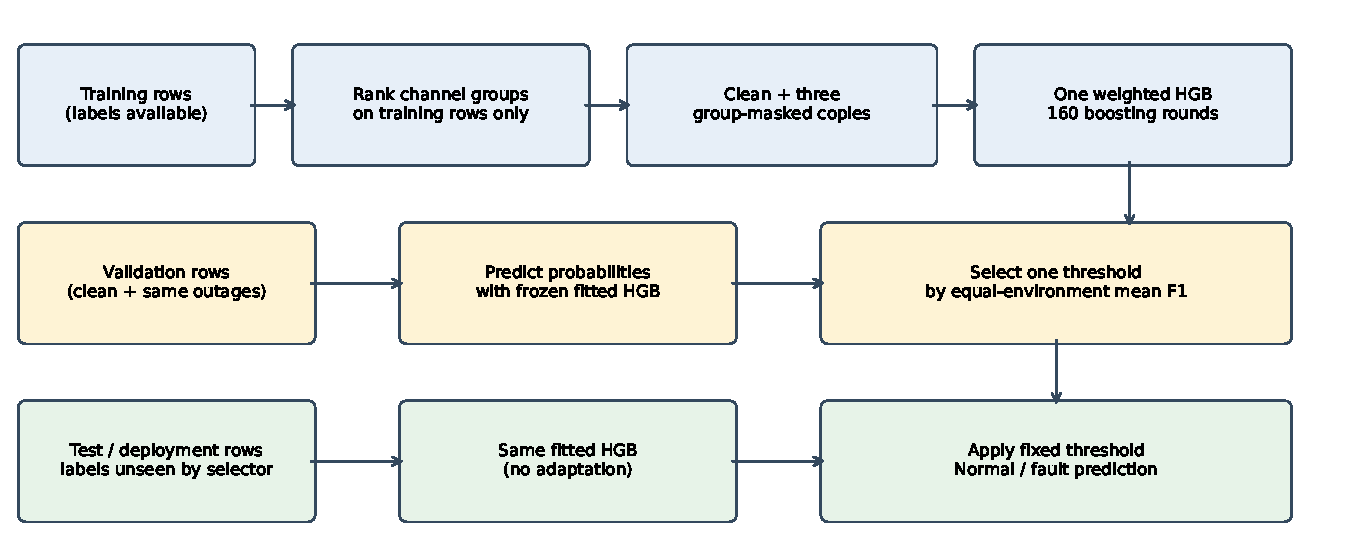
\includegraphics[width=.95\textwidth]{figures/architecture.pdf}
\caption{The Group-HGB workflow. Blue blocks fit the predictor, yellow blocks choose a decision threshold, and green blocks apply frozen components. Standard HGB removes augmentation; Cell-HGB replaces whole-group training masks with matched-budget cell masks.}
\label{fig:architecture}
\end{figure*}

\subsection{Evaluation environments and statistics}
Each fitted model is evaluated on eight conditions: clean; one complete outage for each top-five group; and independent cell masking at 10\% and 30\%. All methods share the same test rows and corruption masks within a split. Because we remove measurements from an existing test table, these are controlled interventions, not observed histories of equipment outages.

The primary endpoint averages positive-class F1 over clean and three development-family outages. These are anticipated outage identities on unseen rows. The two additional group outages evaluate transfer to outage identities omitted from deliberate augmentation and threshold tuning. MCAR conditions provide a separate mechanism check.

Results report the mean and sample standard deviation across split seeds. APS runs share the same test rows; they are not three independent fleets. For the primary Group-HGB minus HGB contrast, we compute 1,000 paired, class-stratified row-bootstrap replicates. APS replicates resample the same rows jointly across all seeds and environments. For AI4I, the bootstrap uses the predesignated first seed only because the three test sets differ. Its interval must not be attached to the three-split mean. These intervals condition on the fitted models, observed class proportions, and benchmark; they do not quantify uncertainty across fleets or datasets.

\section{Result and Analysis}
\subsection{Metrics}
With fault as the positive class,
\begin{align}
 \mathrm{Accuracy}&=\frac{TP+TN}{TP+TN+FP+FN},\\
 \mathrm{Precision}&=\frac{TP}{TP+FP},\qquad
 \mathrm{Recall}=\frac{TP}{TP+FN},\\
 F_1&=\frac{2TP}{2TP+FP+FN}.
\end{align}
A zero denominator gives zero for the corresponding precision, recall, or F1. For class-specific scores $F_{1,c}$ and support $n_c$,
\begin{equation}
 F_{1,\mathrm{macro}}=\frac12\sum_{c=0}^{1}F_{1,c},\quad
 F_{1,\mathrm{weighted}}=\sum_{c=0}^{1}\frac{n_c}{n}F_{1,c}.
\end{equation}
Macro and support-weighted precision and recall are computed similarly. We also report average precision (AP; scikit-learn's non-interpolated summary of the precision--recall curve), AUROC, confusion matrices, false positives per 1,000 negative records, and the APS diagnostic cost. AP is not a trapezoidal PR-AUC calculation.

\begin{table*}[t]
\centering\caption{Clean-test classification results, mean over three fixed split seeds. Metrics are percentages except AP, which is on $[0,1]$. These are our runs, not cross-paper comparisons.}
\label{tab:clean}\small
\begin{tabular}{llrrrrrrr}\hline
Dataset & Model & Accuracy & Precision & Recall & $F_1$ & Macro $F_1$ & Weighted $F_1$ & AP\\\hline
APS & Logistic & 98.84 & 76.14 & 75.47 & 75.41 & 87.41 & 98.84 & 0.828\\
APS & HGB & 99.28 & 87.91 & 80.36 & 83.88 & 91.75 & 99.26 & 0.916\\
APS & Group-HGB & 99.30 & 88.63 & 80.62 & 84.36 & 92.00 & 99.28 & 0.912\\
AI4I & Logistic & 93.98 & 18.04 & 21.57 & 19.61 & 58.24 & 94.25 & 0.159\\
AI4I & HGB & 97.63 & 66.96 & 66.18 & 65.76 & 82.27 & 97.65 & 0.759\\
AI4I & Group-HGB & 98.13 & 77.80 & 64.22 & 70.08 & 84.56 & 98.05 & 0.734\\
\hline\end{tabular}\end{table*}

\begin{table}[t]\centering\caption{Positive-class $F_1$ over clean plus three development-family outage environments. Mean $\pm$ sample SD over three split seeds. ``Env'' selects a threshold using all four validation environments.}\label{tab:ablation}\small
\begin{tabular}{llrr}\hline
Training & Threshold & APS & AI4I\\\hline
Logistic & Clean & $0.659\pm0.018$ & $0.139\pm0.012$\\
HGB & 0.5 & $0.782\pm0.013$ & $0.542\pm0.021$\\
HGB & Clean & $0.836\pm0.014$ & $0.561\pm0.020$\\
HGB & Env & $0.836\pm0.014$ & $0.565\pm0.024$\\
Group-HGB & 0.5 & $0.783\pm0.008$ & $0.485\pm0.014$\\
Group-HGB & Clean & $0.843\pm0.008$ & $0.604\pm0.015$\\
Group-HGB & Env & $0.843\pm0.008$ & $0.601\pm0.017$\\
Cell-HGB & Env & $0.839\pm0.012$ & $0.598\pm0.004$\\
\hline\end{tabular}\end{table}

\begin{table}[t]\centering\caption{Transfer to untrained full-group outages (G4/G5), averaged over both groups and all three split seeds. Random cell masking is a control, not a newly proposed algorithm.}\label{tab:transfer}\small
\begin{tabular}{lrr}\hline
Model & APS $F_1$ & AI4I $F_1$\\\hline
Logistic & 0.712 & 0.207\\
HGB & 0.839 & 0.488\\
Group-HGB & 0.843 & 0.404\\
Cell-HGB & 0.841 & 0.582\\
\hline\end{tabular}\end{table}


\subsection{Clean performance and anticipated outages}
On clean APS, Group-HGB reaches 99.30\% accuracy, 88.63\% precision, 80.62\% recall, and F1 0.844 (Table~\ref{tab:clean}). Standard HGB achieves F1 0.839 and AP 0.916, compared with Group-HGB's AP 0.912. A small F1 increase therefore does not establish better ranking quality. The majority classifier achieves 97.66\% accuracy on this test set but zero positive-class recall and F1.

For the primary four-environment average, APS Group-HGB obtains $0.8435\pm0.0076$ versus $0.8359\pm0.0137$ for standard HGB. The paired difference is 0.0076 with a conditional 95\% bootstrap interval $[-0.0010,0.0166]$. This experiment does not establish a reliable improvement on the real dataset.

AI4I shows a larger mean increase: $0.6006\pm0.0166$ versus $0.5610\pm0.0205$. For seed 11 specifically, the difference is 0.0801 with interval $[0.0178,0.1445]$; this is not an interval for the across-split difference of 0.0396. The contrast between datasets makes a universal benefit claim inappropriate.

\subsection{Threshold selection and matched-cell control}
Table~\ref{tab:ablation} shows that operating points matter. At $t=0.5$, primary AI4I F1 is 0.485 for Group-HGB and 0.542 for HGB. Under their clean-selected thresholds, the ordering reverses: 0.604 versus 0.561. Reporting only one favorable threshold would hide this dependence.

Environment-aware threshold selection adds no primary gain to APS HGB or Group-HGB because it selects the same thresholds as the clean policy. For AI4I it changes Group-HGB's primary mean from 0.604 to 0.601. Thus, the anticipated-outage advantage cannot be credited to that threshold policy. Cell-HGB with an environment threshold reaches 0.598 on AI4I, close to Group-HGB's 0.601. The first-seed Group-HGB minus Cell-HGB bootstrap interval, $[-0.0132,0.0650]$, also spans zero. Targeted group masking is not established as superior to the matched-cell control.

A further, explicitly post-hoc control fits the same learner on four identical clean copies with quarter weights. This preserves total row weight while changing representation counts, which can affect minimum-leaf constraints and histogram construction. Across the same four test environments, clean-repeat HGB with an environment-selected threshold reaches $0.8365$ on APS and $0.6136$ on AI4I. The latter exceeds Group-HGB's $0.6006$. Thus, even the observed AI4I advantage over the original HGB cannot be attributed specifically to the targeted masks. These six extra fits were declared after identifying the count constraint and are archived separately from the original 24-fit experiment; they do not replace the confirmatory comparison. A future confirmatory design should include this control from the outset.


\subsection{Failure to transfer}
\begin{figure*}[t]
\centering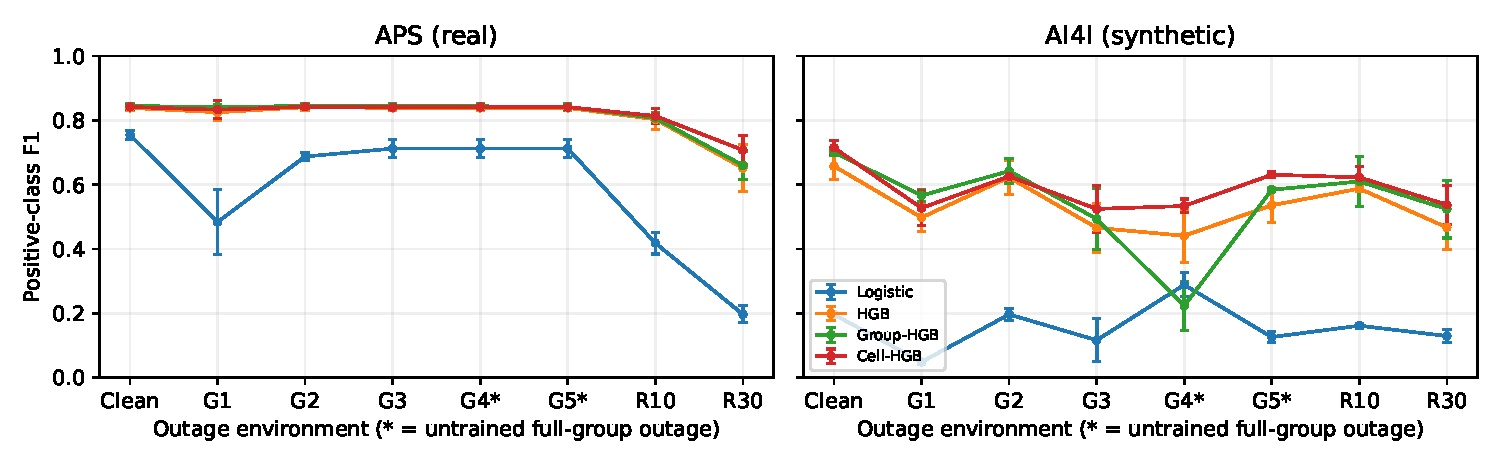
\includegraphics[width=.96\textwidth]{figures/outage_f1.pdf}
\caption{Positive-class F1 by environment. Points are three-split means; error bars are sample standard deviations, not confidence intervals. G1--G3 were used in development; G4/G5 were excluded from deliberate group augmentation and threshold tuning. R10/R30 denote random-cell removal rates. Group identities may change with the training split.}
\label{fig:outages}
\end{figure*}

The untrained AI4I outages expose a clear limit (Table~\ref{tab:transfer}). Average G4/G5 F1 is 0.404 for Group-HGB, 0.488 for standard HGB, and 0.582 for Cell-HGB. In all three splits, G4 is rotational speed. Removing it reduces Group-HGB's F1 to 0.223 and recall to 0.132, compared with standard HGB's F1 0.441. Its 96.92\% accuracy remains superficially high because most records are negative. A model can therefore improve on anticipated outages while losing substantial minority detection on a different outage.

Under 30\% random-cell masking, APS Group-HGB reaches F1 0.660, compared with HGB's 0.652. Both are substantially below their clean results. AI4I values are 0.524 and 0.467. These results concern the specified synthetic masks; they do not estimate the frequency or cost of real sensor failures.

\subsection{Redundancy, diagnostic cost, and computation}
A post-fit training-only audit finds near-perfect observed-value correlations among APS variables \texttt{bb\_000}, \texttt{bv\_000}, \texttt{cq\_000}, and \texttt{bu\_000}. These occupy four of the top-five ranks for seed 11, whereas \texttt{ci\_000} ranks first. Their separate deletion can preserve almost the same information through another counter. Prefix grouping therefore does not guarantee an information-level outage. This limits interpretation of the small APS gap.

We also run an explicitly exploratory joint-deletion sensitivity after fixing its procedure in a separate file. On each training split, top-five single-column groups with absolute Pearson correlation above 0.9999 form connected components (at least 1,000 jointly observed rows). The first non-singleton component is deleted jointly from the official test data, using the existing models and thresholds. No model is retrained. Results are retained separately; this post-hoc check is not counted as confirmatory evidence or evidence that the counters share a physical sensor.

Optimizing F1 also changes the application tradeoff. On clean APS, standard HGB's F1-selected threshold yields mean diagnostic cost 37,253, compared with 20,370 at $t=0.5$. Group-HGB gives 36,727 versus 19,677. The cost weights penalize missed faults heavily, while F1 does not use those weights. A higher F1 is therefore insufficient evidence of lower operational cost.

All 24 principal/control fits together take 88.7 seconds of measured fit time in this environment, excluding acquisition, evaluation, analysis, and reproduction checks. APS HGB averages 2.61 seconds per fit; Group-HGB averages 8.71 seconds. Compressed Group-HGB artifacts are approximately 210 kB, similar to HGB. Augmentation increases fitting time but retains one predictor at inference. These timings demonstrate feasibility on this CPU instance, not a guaranteed Colab or laptop runtime.

\begin{figure}[t]
\centering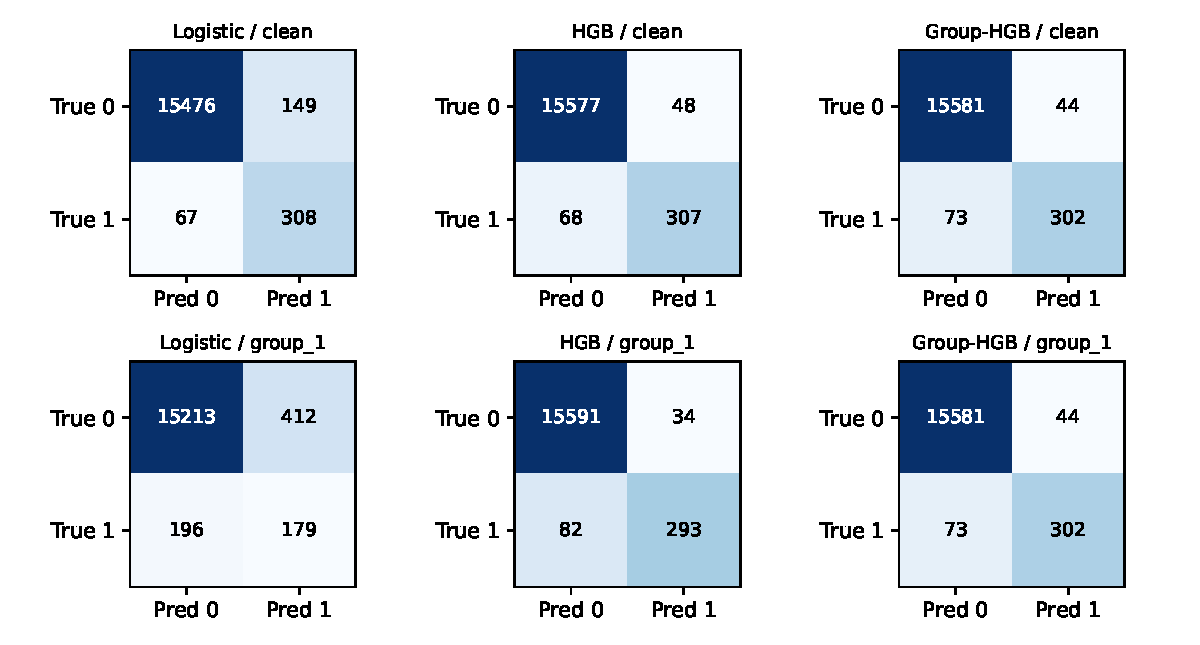
\includegraphics[width=\columnwidth]{figures/confusion.pdf}
\caption{Confusion matrices on the fixed APS seed-11 test, clean data and G1 outage. Counts show the minority errors that aggregate accuracy can conceal. The color scale is logarithmic; printed values are raw counts.}
\label{fig:confusion}
\end{figure}

\section{Conclusion}
Group-outage augmentation improves the anticipated-outage mean on synthetic AI4I, but the real APS gain is small and its conditional uncertainty includes zero. Its AI4I advantage largely disappears against matched random-cell masking and reverses on the untrained rotational-speed outage. Outage identities and threshold policy must therefore accompany any claim of improved missing-input performance. The strongest practical result is the transfer failure and the usefulness of retaining a cheap corruption control, rather than a universally better classifier.

\section{Discussion}
This study contributes a runnable comparison with artifacts that allow a reader to inspect exactly which records, masks, scores, thresholds, and errors produced each result. It provides a useful course research project and a narrow empirical case study. It does not establish that Group-HGB is a new algorithm, that this combination is absent from all prior work, or that the observed findings generalize to industry.

Several limitations matter. Only one real dataset and one synthetic dataset are evaluated. The HGB configuration is shared and fixed; tuned random forests, XGBoost, missingness-avoiding trees, and recent neural or foundation models are not reproduced. Correlated APS counters weaken single-variable stress, and anonymized groups do not identify physical acquisition units. AI4I random partitions cannot establish prospective temporal generalization. Each MCAR rate uses one fixed draw per split, so mask-to-mask variability is not independently characterized. Three split seeds provide limited information about training variability; test-row bootstrap intervals condition on fitted models and do not address it fully.

Finally, equal-environment F1 implicitly assigns equal weight to clean inputs and each planned outage. Real deployments need observed outage frequencies, severity, class prevalence, and diagnostic costs. Future work should use known acquisition groups, natural longitudinal outages, more independent datasets, and nested development experiments that hold out entire outage families. A cost-sensitive threshold and a broader, validation-selected augmentation distribution are reasonable hypotheses for that work. They are not claimed as results of this experiment.

\bibliographystyle{IEEEtran}
\bibliography{references}
\end{document}
